\documentclass[11pt]{article}
% \pagestyle{empty}

\setlength{\oddsidemargin}{-0.25 in}
\setlength{\evensidemargin}{-0.25 in}
\setlength{\topmargin}{-0.9 in}
\setlength{\textwidth}{7.0 in}
\setlength{\textheight}{9.0 in}
\setlength{\headsep}{0.75 in}
\setlength{\parindent}{0.3 in}
\setlength{\parskip}{0.1 in}
\usepackage{epsf}
\usepackage{pseudocode}
\usepackage{ amssymb }
\usepackage{tikz}
\usepackage{listings}
\usetikzlibrary{arrows.meta}
\usepackage{algorithmic}
\usepackage{changepage}
\usepackage{lipsum}
\usepackage{enumitem}
\usepackage{indentfirst}
\pagestyle{headings}
\usepackage{graphicx}
\graphicspath{ {desktop/} }


% \usepackage{times}
% \usepackage{mathptm}

\def\O{\mathop{\smash{O}}\nolimits}
\def\o{\mathop{\smash{o}}\nolimits}
\newcommand{\e}{{\rm e}}
\newcommand{\R}{{\bf R}}
\newcommand{\Z}{{\bf Z}}
\newcommand{\findent}{\leavevmode{\parindent=2em\indent}}
\newcommand\solution{%
  \textbf{Solution.}\\%
}
\begin{document}

CS 124 Programming Assignment 2 \\
\indent HARVARD IDs: 10939860 60950350
\\

\textbf{Introduction:}\\
This write-up discusses our theoretical analysis, experimental analysis, and programming implementation of Strassen's Algorithm for matrix multiplication. We will first walk through how we mathematically solved for optimal cross-over points using recurrence and running times, and distinguishing between the cases for even and odd dimensions. Then we will represent our experimental analysis with tables and graphs and include an analysis of those numbers and the differences we found between the two analyses. Finally, we will explain the process we took to implement the algorithm and the decisions we made to try to optimize our code, and discuss our final conclusions for the assignment. \\\\


\textbf{Theoretical Analysis:} \\\\
We calculated the cross-over point by considering the runtime for traditional matrix multiplication and the recurrence equation for the modified version of Strassen's algorithm. Let $M(n)$ be the runtime for the traditional matrix multiplication algorithm. Our first equation says that: \\
$M(n) = (2n - 1)n^2$ \\
This is because there are $n^2$ dot products to compute for matrix multiplication, one dot product for every cell in an $n$ x $n$ matrix, and for each of those dot products there are $n$ multiplications and $n - 1$ additions to compute. Putting this together, you get $n^2(n + n - 1)$ = $(2n - 1)n^2$. \\\\
Let $S(n)$ be the recurrence equation for Strassen's algorithm. Our second equation gives: \\
$S(n) = 7S(\lceil n/2\rceil) + 18(\lceil n/2 \rceil)^2$ \\\\
This recurrence was derived by counting the number of multiplications, additions, and subtractions used in Strassen's algorithm. When computing the seven products that define Strassen's, there are a total of 7 multiplications, each done on matrices of size $\lceil n/2 \rceil$ based on the recursion in the algorithm, and a total of 18 matrix additions and subtractions, also each on matrices of size $\lceil n/2 \rceil$. Since adding or subtracting matrices takes one computation for each cell in the matrix, which is the dimension squared, we must square the last $\lceil n/2 \rceil$ in the equation. The ceiling function is necessary for this recurrence equation because the algorithm is based on recursing over submatrices that are half the dimension of the original, but splitting matrices up in this way only works for matrices of an even dimension. The way Strassen's algorithm can be implemented to account for this, and as we have implemented in our own code, is to pad the matrices with one row and one column of zeros if the dimension is an odd number. Doing this would mean that the recursion would be over matrices of dimension $(n + 1)/2$, which is what the ceiling function would give. \\\\
With these two equations, we can find the crossover point by combining both in such a way that will switch over to the traditional multiplication runtime when that becomes optimal. This can be represented in a piecewise function. Let $T(n)$ be the recurrence equation for the modified version of Strassen's: \\
$T(n) = \{$ \\
$T(\lceil n/2 \rceil) + 18(\lceil n/2 \rceil)^2$ if $n > n_0$ \\
$M(\lceil n/2 \rceil)$ otherwise $\}$ \\
This means that the modified Strassen's will work as a normal Strassen's algorithm until some point $n_0$, at which point it switches to the traditional multiplication. \\\\
We want this switch the occur at the most optimal time, which will be when Strassen's begins to run slower than the traditional method -- when $S(n) \geq M(n)$. To find this point, therefore, we can set the two equations equal together and solve for $n$: \\
$(2n - 1)n^2 = 7(2\lceil n/2 \rceil - 1)(\lceil n/2\rceil^2) + 18(\lceil n/2\rceil^2)$ \\\\
Because this equation requires ceilings, at this point it is necessary to distinguish between even values of $n$ and odd values of $n$. In the even case, $\lceil n/2 \rceil$ = $n/2$, so we can simply take out all the ceiling functions and calculate the equation like that. Plugging this into a calculator, we get $n = 15$. Since we are just looking at even values for $n$ in this case, we round up to the nearest even number and get $n = 16$ as the optimal cross-over point for even $n$. \\\\
For the odd case, we can let $n = 2k + 1$, since this will be a valid equation for odd integer $n$ and any integer $k$. Using the padding method of adding one row and column of zeros on any odd-dimension matrix, we see that all instances of $\lceil n/2 \rceil$ will be substituted for $\lceil (2k + 1)/2 \rceil$, which simplifies to $\lceil k + (1/2) \rceil$ = $k + 1$. Plugging this back into the equation and solving with a calculator, we get that $k = 18.085$ and therefore $n = 37.17$. We then want to round this value up to the nearest odd number, since we are only dealing with odd numbers in this case, giving $n = 39$ as the optimal cross-over point for odd $n$. \\\\

\textbf{Experimental Analysis:} \\
To test the cross-over point experimentally with our code, we ran the algorithm for a variety of cross-over points and recorded the time it took to run each. For every time shown in the data below, it is the average of 5 trials running on the same dimension and cross-over. We set the dimension to be 128 because it was a reasonably medium-sized matrix to test, and also because we noticed that the times were all about the same for any dimension. In order to create our ASCII files for the matrices, we randomly generated $2*(dimension)^2$ numbers between 1 and 10. \\\\
For the cross-over points, we tested every tenth number from 1 to 150 (1, 10, 20, ..., 150). We noticed that at some point the time began to even out and plateau, so we tested the algorithm on dimension 500 to see if it was still the same. The time it took for dimension 500 was the same as it took in the 100-150 range, so at this point we concluded that the time continues to plateau for all dimensions after our cross-over point. \\\\
We knew that the time for even dimensions and odd dimensions would differ as a result of the padding and extra code running for that, so we completed the same process to test for cross-over points with the odd dimension 129. We ran the same cross-over points, averaging the time for 5 trials each, and recorded. \\\\
The numeric results of our experimental analysis are shown in the following tables and graphs: \\\\\\\\\\\\\\\\\\\\
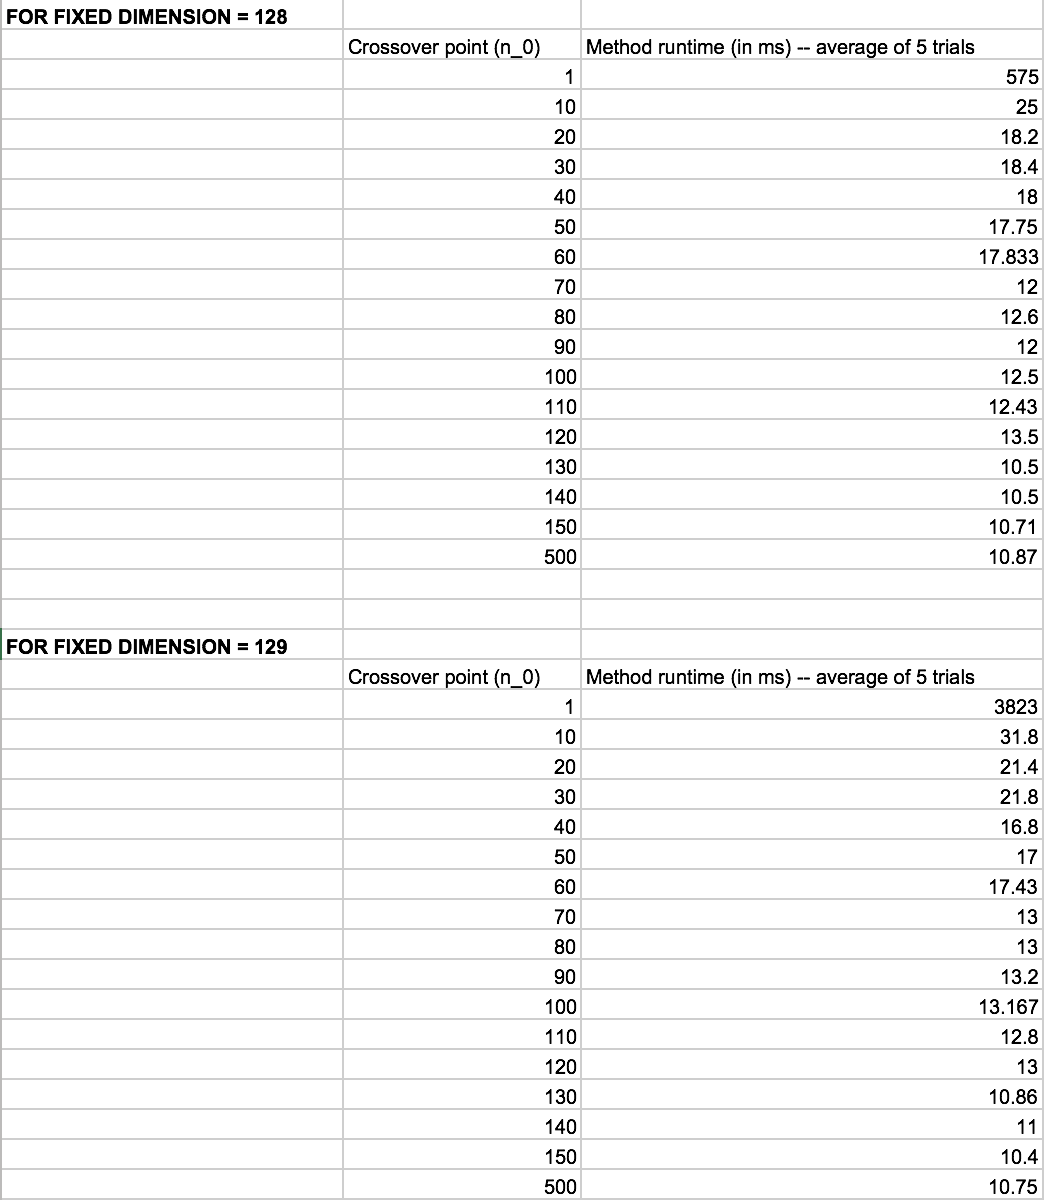
\includegraphics{runtimetable}
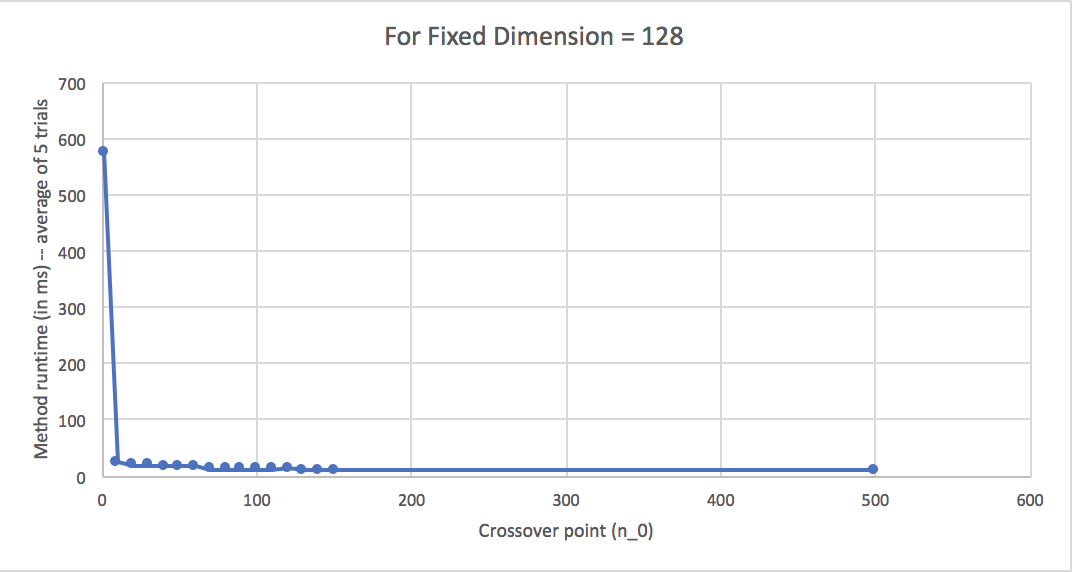
\includegraphics{128graph}
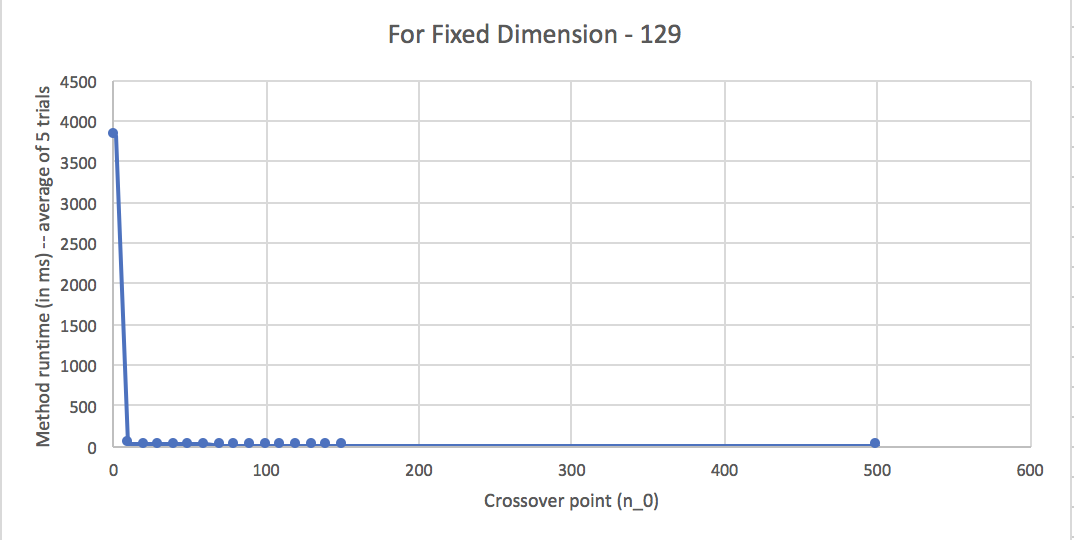
\includegraphics{129graph}

Based on the tables and graphs, we concluded that the code's optimal cross-over point was approximately $n = 130$ for even dimensions and approximately $n = 131$ for odd dimensions. Both times plateaued around 11 milliseconds, which was the shortest time we ever recorded, so the cross-over point was where that trend began. \\\\
These results were fairly surprising, given that we had completed and understood the theoretical analysis first, and assumed we would find a similar result around 16 and 39. Our odd case ran significantly slower than the even case for smaller cross-over values, which makes sense since this would mean that a layer of padding would need to be added many more times. When the cross-over point was higher, there were fewer and at some point no padding steps necessary. This is when the values align exactly with the even case, which also makes sense. \\\\
Since our lowest time was for cross-over values that were greater than the dimension size, this means that the fastest case was actually when all the multiplication was done using the traditional multiplication method, not Strassen's. This, of course, is not what should happen in theory, which we can understand from the lecture on Strassen's as well as our specific findings in the theoretical analysis. We understood this as a sign that our implementation of Strassen's algorithm was not fully optimal, and therefore the naive multiplication was still faster. We are not yet confident in exactly what part of the code caused the algorithm to run slower than it should, but we have considered that it is a result of making new 2D arrays for every recursion on strassens and for copying in a lot of different information to new arrays. Our implementation will be discussed in further detail below. \\\\




\textbf{Implementation Details:} \\ (note: "make" will compile our code, but you can only run it with "java strassen $<$flag$>$ $<$dimension$>$ $<$inputfile$>$" -- thank you!)\\\\
We used Java to implement the code for this algorithm, taking advantage of its ability to pass arrays between functions, avoiding the need to allocate and deallocate lots of memory, and for the simplicity of dealing with these types in general (all issues that we would otherwise have faced with C). For Strassen's algorithm, we implemented matrices as 2D arrays. In a separate file, we read the ASCII text and write the information into two 2D arrays that are then both put into a size 2 matrix, and passed to the $strassen$ file. Dealing with these types was perhaps the most complicated part of the code for us -- we needed the $Matrix$ file to output a matrix, but we needed the contents of that matrix to be a 2D array that $strassen$ would then be able to handle. At the top of the $strassen$ file, we convert the matrix from $Matrix$ into two 2D arrays, which are then immediately run on the $strassens$ function. \\\\
Implementing the recursion on Strassen's algorithm was relatively easy. Understanding that we would need to pad our matrices with zeros for odd dimensions, we chose to split up our $strassen$ function in a few cases: 1) depending on the cross-over point, if the dimension is less than the cross-over, simply run the traditional matrix multiplication function on the matrices and return that; 2) if the dimension is even, then Strassen's can currently recurse on that, so recurse; and 3) if the dimension is odd, pad with one row and column of zeros and recurse over that. \\\\
With even dimensions, for the sake of simplicity, we chose to create 8 new 2D arrays, 4 for each matrix $A$ and $B$, and copied the correct numbers from $A$ and $B$ to the submatrices. We then recurse in the definition of the $p$ values for Strassen's 7 products. Finally, we put that information back into 4 submatrices and then into the final answer matrix, $product$. \\\\
In the odd case, we believed that the minimal amount of padding possible to add to make the function work correctly, and therefore the optimal amount of padding, would be to just add one row and one column of zeros any time the dimension is odd. Padding in this way means that every time the dimension is odd, create a new matrix of dimension $n + 1$ and add in the information from the original matrix. The other option we considered was pad to the next power of two any time the dimension was either odd or any time it was not a power of two. This meant, however, that many more zeros would have to be added at once, which could often lead to more padding than necessary. We were also following the analytic conclusion we had found, which relied on doing the 1-zero pad method. To get rid of the padding at the very end, when we copy the information to $product$, we will only run our loop until the original dimension size, meaning that the last row and column of zeros would be lost. \\\\
This implementation proved to be quite time efficient, taking less than one second to run for most matrix sizes we tested, up until about dimension 1024, at which point it took only barely over one second (not including the time to print the result). \\\\ 

\textbf{Conclusion:} \\
Although our Strassen's code is perhaps not the most optimal implementation, we have concluded that our implementation is correct and fully functional, and not too far from the time that it should be. We believe that our padding was optimal and that our treatment of the 7 products is as it should be. The naive multiplication algorithm appears to be more time efficient than Strassen's based on our experimental analysis, we think that our Strassen's algorithm is still running in a normal, relatively quick speed (based on discussions in office hours with TFs and classmates). Even for cross-over 1, when Strassen's runs on its own, an even dimension matrix takes less than a second to run and an odd dimension matrix takes about four seconds. Though it is not perfect, we have gained a much fuller understanding of Strassen's algorithm and the ideal cross-over points for matrix multiplication, and have worked hard to get an accurate and reasonably fast implementation. 

\end{document}
